% Im Juni 2000 stellte das Unternehmen Microsoft das \ac{dotnet} vor.
% Kurz darauf wurde von Miguel de Icaza das sogenannte Mono-Projekt als Open-Source gestartet, welches eine Linux-Version des \ac{dotnet} darstellen soll.
% Am 16. Mai 2011 kündigt Miguel de Icaza an, dass das Mono-Projekt vom Unternehmen Xamarin weiterentwickelt wird, wobei einige wichtige Mitglieder des Mono-Entwickler-Teams weiterhin daran beteiligt sind.

% Das Unternehmen Xamarin wurde mit der Absicht gegründet, Software auf mobile Geräte zu vertreiben. 
\label{ch:prog-doc}
\section{Übersicht}
Das im Zuge dieser Diplomarbeit entwickelte Software-Projekt basiert auf einer der von Microsoft bereitgestellten Xamarin.Forms-Vorlagen, welche als Teil von Visual Studio bereitgestellt werden.
Es gibt mehrere Auswahlmöglichkeiten, wobei alle Vorlagen bis auf \enquote{Blank} Beispielcode beinhalten.
Da der Beispielcode der anderen Vorlagen für dieses Projekt nicht relevant ist und ohnehin gelöscht werden müsste, wird die \enquote{Blank}-Vorlage verwendet.
Diese Vorlage beinhält nur eine Haupt-Oberflächenseite ohne jeglichen Beispielcode.

Der immer wieder vorkommende Name PiBell ist eine freigeistliche Erfindung. PiBell ist der Projektname, der sich aus \acl{rpi} und \enquote{Bell}, dem englischen Wort für Klingel oder Glocke, zusammensetzt.

Visual Studio organisiert alle Programmteile in einer sogenannten Solution, welche den Projektnamen trägt. In diesem Fall beinhält die Solution \enquote{PiBell} drei Programmteile oder \enquote{Projects}:
\paragraph{PiBell} ist das portable Projekt, auch .NET-Standard-Projekt genannt.
Dieses beinhaltet den ganzen plattformunabhängigen Code, sowie die Definition der UI-Oberfläche mittels XAML-Dateien.
In diesem Projekt befindet sich der größte entwickelte Code-Anteil, da die meisten Funktionen, wie das Abspielen von Videos mit Hilfe der LibVLC-Bindings, plattformunabhängig funktionieren und deswegen geteilt werden können.

\paragraph{PiBell.Android} beinhaltet allen Code, der plattformspezifisch für Android geschrieben wurde.
Unter anderem ist hier enthalten die Android-Implementation des Mikrofon-Auf\-nahme-Services, sowie das Berechtigungs-Management.
Die Mikrofon-Aufnahme erfolgt auf einer sehr hardwarenahen Ebene, was die plattformabhängigkeit erklärt.

\paragraph{PiBell.iOS} beinhaltet wie PiBell.Android den plattformspezifischen Code für die iOS-Platt\-form. Aufgrund mangelnder Entwicklungswerkzeuge wurde dieser Teil nicht großartig behandelt.\par

\begin{figure}[H]
\centering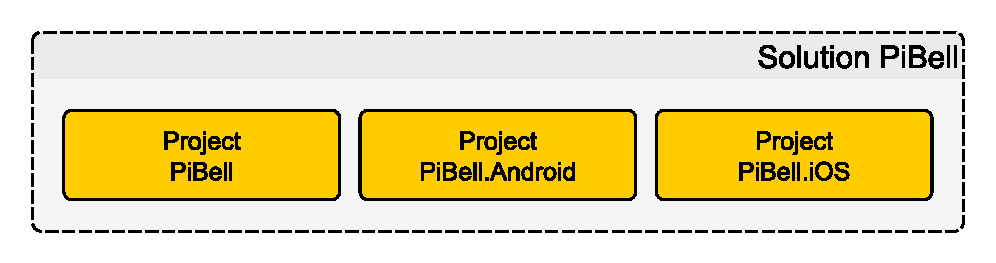
\includegraphics[width=0.9\linewidth]{images/xamarin/struktur.pdf}
\caption{Aufbau der Solution}
\end{figure}

%besteht aus drei teilen
%- portable project/.net standard project
%   plattformunabhängiger teil, oberfläche, ...
%- Android project
    %android-spezifischer teil, berechtigungen, ...
%- iOS project
    %iOS-spezifischer Teil, ...
%project-name PiBell -> erfindung, leitet sich aus raspberry und Türglocke ab
%
\section{Portable Project}
\section{PiBell.Android}
\section{PiBell.iOS}